% Anonymized main document for Network Science double-blind review.
% Compile from this directory: pdflatex, bibtex, pdflatex, pdflatex.
\documentclass{nws}

\usepackage{amsmath,amssymb,booktabs,graphicx}
\usepackage[hidelinks]{hyperref}
\usepackage{microtype}
\renewcommand{\toprule}{\hline}
\renewcommand{\midrule}{\hline}
\renewcommand{\bottomrule}{\hline}

\lefttitle{Directed Link and Hyperlink Prediction}
\righttitle{Network Science}
\papertitle{Research Article}
\jnlPage{1}{1}
\jnlDoiYr{2026}
\doival{to be assigned}
\title{Exponential Random Graph Models as a Statistical Benchmark for Directed Link and Hyperlink Prediction in Legislative Co-sponsorship}
\author{Anonymous}
\affil{Blinded for review}

\begin{document}

\begin{abstract}
Public political records frequently encode a group relation with ordered roles: for a Senate bill, one legislator is the sponsor and a set of legislators are original co-sponsors. Its familiar directed dyadic projection preserves sponsor--co-sponsor arcs but loses the partition of arcs into recorded coalitions. We develop a missingness-centred benchmark that keeps three prediction targets distinct: recorded ordered group-event types, directed dyadic footprints, and algebraically derived formal concepts from the aggregate projection. Using 4,374 nonempty-head Senate bills from the 118th Congress, we mask whole sponsor-to-original-co-sponsor event types under random and activity-biased mechanisms, fit split-specific directed ERGM pseudolikelihood models, and compare their conditional footprint scores with transparent directed local statistics. Formal concepts do not recover recorded coalitions: the cap-first Senate audit yields zero exact ordered matches and a footprint Jaccard similarity of 0.048. ERGM conditionals markedly exceed a density-only reference on random panels, yet directed local references outperform the ERGM on both random and grammar-preserving sponsor-substitution panels. Fixed-participant sponsor identification produces the same qualitative separation. The result is therefore a benchmark, rather than a universal claim of ERGM superiority: the inferential object, candidate panel, and ordered role grammar jointly determine what a score can establish. Enron email and MathOverflow exchanges provide contrasting non-political scope checks. The analysis concerns controlled omissions in complete public records; it does not estimate archival missingness or forecast future legislation.
\end{abstract}

\begin{keywords}
political networks; legislative co-sponsorship; exponential random graph models; hyperlink prediction; missing network data; directed hypergraphs
\end{keywords}

\maketitle

\section{Introduction}\label{sec:introduction}

Political networks are frequently built by projecting a public record of collective action into dyadic ties. This practice is useful, but it can obscure the object to be predicted. In a Senate bill record, a sponsor and the bill's original co-sponsors form a directed group relation, whereas a sponsor--co-sponsor projection records only the constituent directed arcs. The projection cannot say which arcs constituted the same bill coalition. Co-sponsorship is a prominent and substantively interpretable political relation \citep{fowler2006,talbertPotoski2002,zhangEtAl2008}; the measurement issue also arises for treaty signatories, joint statements, amicus coalitions, and diplomatic exchanges. In each case, a recorded group, its dyadic footprint, and a group derived from that footprint are different mathematical objects.

This distinction matters for political-network inference as well as for prediction. A scholar may want to recover a missing directed tie in a projected network, to rank a missing recorded coalition type, or to study a closed group structure implied by the aggregate relation. These tasks can share nodes and directed arcs while having different response variables, candidate spaces, and notions of success. Treating them as interchangeable creates a particularly misleading comparison when a high score on easy random alternatives is read as evidence of recovering sponsors, coalition membership, or political leadership.

We ask how a directed exponential random graph model (ERGM) can serve as a statistical benchmark for directed link and hyperlink prediction when observations are deliberately made incomplete. The application is the completed 118th United States Senate, where the public Bill Status record identifies one sponsor and the original co-sponsors of each Senate bill. The benchmark has four contributions. First, it makes the target ladder explicit by distinguishing native coalition types, directed dyadic footprints, and formal concepts derived from the footprint. Second, it provides an event-first controlled-missingness design in which all copies of a selected native event type are withheld together. Third, it compares split-specific ERGM conditional footprint scores with directed local statistics under the same masks and candidate panels. Fourth, it turns direction into a political question: among the legislators recorded on a bill, can a score identify the sponsor rather than merely exploit aggregate popularity or coalition size?

The approach connects link prediction \citep{libenNowellKleinberg2007,luZhou2011,zhaoEtAl2017}, higher-order closure \citep{bensonEtAl2018}, and research on network missing data \citep{kossinets2006,handcockGile2010,koskinenEtAl2010}. It does not interpret an absent Senate record as evidence of an unknown natural missing-data process. Instead, controlled omissions define a transparent stress test. ERGMs provide a principled language for directed structural dependence \citep{wassermanPattison1996,robinsEtAl2009,snijdersEtAl2006}, and are established tools in political-network analysis \citep{cranmerDesmarais2011}. Here they are used as conditional-score benchmarks: a fitted model supplies conditional tie scores for an observed training projection, rather than a claimed joint probability of a legislative coalition.

The substantive pattern is deliberately mixed. The aggregate Senate projection generates formal concepts that have zero exact tail/head equality with recorded bill coalitions and only 0.048 footprint Jaccard similarity. The conditional ERGM improves strongly over a density-only reference on random panels, but transparent directed local references are stronger on random and sponsor-substitution panels. The difference is informative rather than contradictory. It shows why a model comparison must identify the missing object and the alternative objects that the score must distinguish. Enron email and MathOverflow exchanges are retained as non-political scope checks, not as equal applications.

\section{Targets, projection, and conditional scores}\label{sec:targets}

\subsection{Recorded events, footprints, and projection non-identifiability}

Let $V$ be a fixed actor universe. A recorded directed group-event type is an ordered pair
\begin{equation}
 e=(T,H), \qquad \varnothing\neq T,H\subseteq V, \qquad T\cap H=\varnothing,
 \label{eq:event}
\end{equation}
where $T$ and $H$ are respectively the tail and head role sets. In the Senate application, $T=\{s_b\}$ contains the sponsor of bill $b$ and $H$ is its set of original co-sponsors. We distinguish an event \emph{type} from repeated occurrences: equal ordered pairs are grouped before masking, so a recurrence cannot remain in the training set after the same type is declared missing.

The directed dyadic footprint of an event is
\begin{equation}
 \phi(T,H)=T\times H,
 \label{eq:footprint}
\end{equation}
and an event collection $\mathcal{E}$ induces a binary directed projection $Y(\mathcal{E})$ with
\begin{equation}
 Y_{ij}(\mathcal{E})=\mathbf{1}\{\exists (T,H)\in\mathcal{E}: i\in T,\ j\in H\}.
 \label{eq:projection}
\end{equation}
Thus the projection records whether an arc occurs in at least one event footprint, but discards its membership partition and multiplicity.

Let $\mathcal{R}$ be the multiset of retained source records. Grouping records with identical ordered role sets gives a type set $\mathcal{E}$ and an occurrence count $c_e$ for each $e\in\mathcal{E}$. The masking unit in this paper is the type, while record-level masking severity weights that type by $c_e$. This distinction matters whenever a source has recurrent groups: withholding one record is not equivalent to withholding the ordered type, because a second identical record would disclose the target.

The loss of information in \eqref{eq:projection} is stronger than the familiar three-actor example. For a loopless directed graph $D=(V,A)$, let $\mathfrak{F}(D)$ be the set of simple directed event collections whose projection is $D$, and define the family of non-dyadic all-ones rectangles
\begin{equation}
 \mathcal{B}(D)=\{(T,H):T,H\ne\varnothing,\ T\cap H=\varnothing,\ |T||H|\geq2,\ T\times H\subseteq A\}.
 \label{eq:projection-fibre}
\end{equation}

\paragraph{Proposition 1 (projection-fibre lower bound).} For every loopless directed graph $D$, $|\mathfrak{F}(D)|\geq2^{|\mathcal{B}(D)|}$. If repeated records or timestamps are part of the representation, the record-level fibre is infinite whenever $A\neq\varnothing$.

\paragraph{Proof.} For every subset $\mathcal{S}\subseteq\mathcal{B}(D)$, construct an event collection containing every singleton arc $(\{i\},\{j\})$ for $(i,j)\in A$, together with every rectangle in $\mathcal{S}$. The singleton events supply all arcs in $A$; every selected rectangle contributes only arcs already in $A$. The projection is therefore $D$ for every $\mathcal{S}$, while distinct subsets produce distinct event collections. This gives the lower bound. Repeating any nonempty event or assigning it a different timestamp leaves the binary projection unchanged, yielding infinitely many record-level representations. \hfill $\square$

The proposition has an important consequence for political records. A perfect dyadic-link predictor can recover the projected arcs and still fail to recover whether those arcs form one co-sponsorship coalition or several distinct bill coalitions. Conversely, a group predictor trained only on a projection is not automatically an estimator of the filed bill record. The event-first benchmark remains well-defined because the evaluator has the source-defined record layer; the predictor is deliberately restricted to information in the observed projection. The benchmark therefore reports results separately for the three targets below.

\subsection{Formal concepts as a third, derived target}

For a binary directed relation $Y$, define the Galois operators for nonempty $T,H\subseteq V$ by
\begin{equation}
 T^{\uparrow}=\{j\in V:Y_{ij}=1\ \text{for every }i\in T\},
 \qquad
 H^{\downarrow}=\{i\in V:Y_{ij}=1\ \text{for every }j\in H\}.
 \label{eq:galois}
\end{equation}
A formal concept is a closed pair $(T,H)$ satisfying $T^{\uparrow}=H$ and $H^{\downarrow}=T$ \citep{ganterWille1999}. Equivalently, it is a maximal all-ones rectangle of the aggregate incidence relation. Formal concepts can be valuable structural descriptions of a co-sponsorship projection. Their status is nevertheless algebraic: closure is defined from all observed arcs in $Y$, not from the bill identifier or the event partition that produced them.

The two derivation operators form a directed Galois connection:
\begin{equation}
 T\subseteq H^{\downarrow}\quad\Longleftrightarrow\quad
 H\subseteq T^{\uparrow}\quad\Longleftrightarrow\quad T\times H\subseteq A(Y).
 \label{eq:galois-connection}
\end{equation}
Thus closure is a relation-level operation. It identifies an inclusion-maximal rectangle even when the arcs entering that rectangle were contributed by several distinct bills, and it can enlarge the role sets of a recorded bill when other bills supply compatible arcs. Because the relation is loopless, a nonempty closed pair cannot place the same actor in both roles: an actor in $T\cap H$ would require its own loop.

It is useful to distinguish the full derived representation from the native event set. One explicit section of the projection map is
\begin{equation}
 f(Y)=\{(\{i\},\{j\}):Y_{ij}=1\}\ \cup\
 \{(T,H): (T,H)\text{ is a formal concept and }|T|+|H|\geq3\}.
 \label{eq:formal-section}
\end{equation}
Every observed arc is present through its singleton event in $f(Y)$, and every formal concept contributes only observed arcs; hence $Y(f(Y))=Y$. This identity makes $f$ a representation of the projection, but it does not make it an inverse of \eqref{eq:projection}. The native event collection can contain different non-singleton groups, record multiplicities, and timestamps while inducing the same $Y$. The concept audit consequently evaluates equality and footprint overlap rather than assuming that a section is a recovered record stream.

For computational and substantive comparability, concept enumeration is cap-first. Given tail and head caps $(c_T,c_H)$, the concept target is
\begin{equation}
 \mathcal{C}_{c_T,c_H}(Y)=\{(T,H):T^{\uparrow}=H,\ H^{\downarrow}=T,
 1\leq |T|\leq c_T,\ 1\leq |H|\leq c_H\}.
 \label{eq:concept-target}
\end{equation}
The cap is applied during enumeration, rather than to an unbounded concept lattice after the fact. Exact event--concept fidelity requires equality of the ordered tail and head sets. Footprint overlap is reported separately because it is a weaker property: it can be high even when no event and concept have the same roles.

Figure~\ref{fig:target-ladder} summarizes the target ladder. The event-first benchmark evaluates recorded bill coalitions, the static directed-arc diagnostic evaluates the projection, and the concept audit asks whether a closure-derived representation corresponds to the bill record. None of these targets substitutes for another.

\begin{figure}[tbp]
\centering
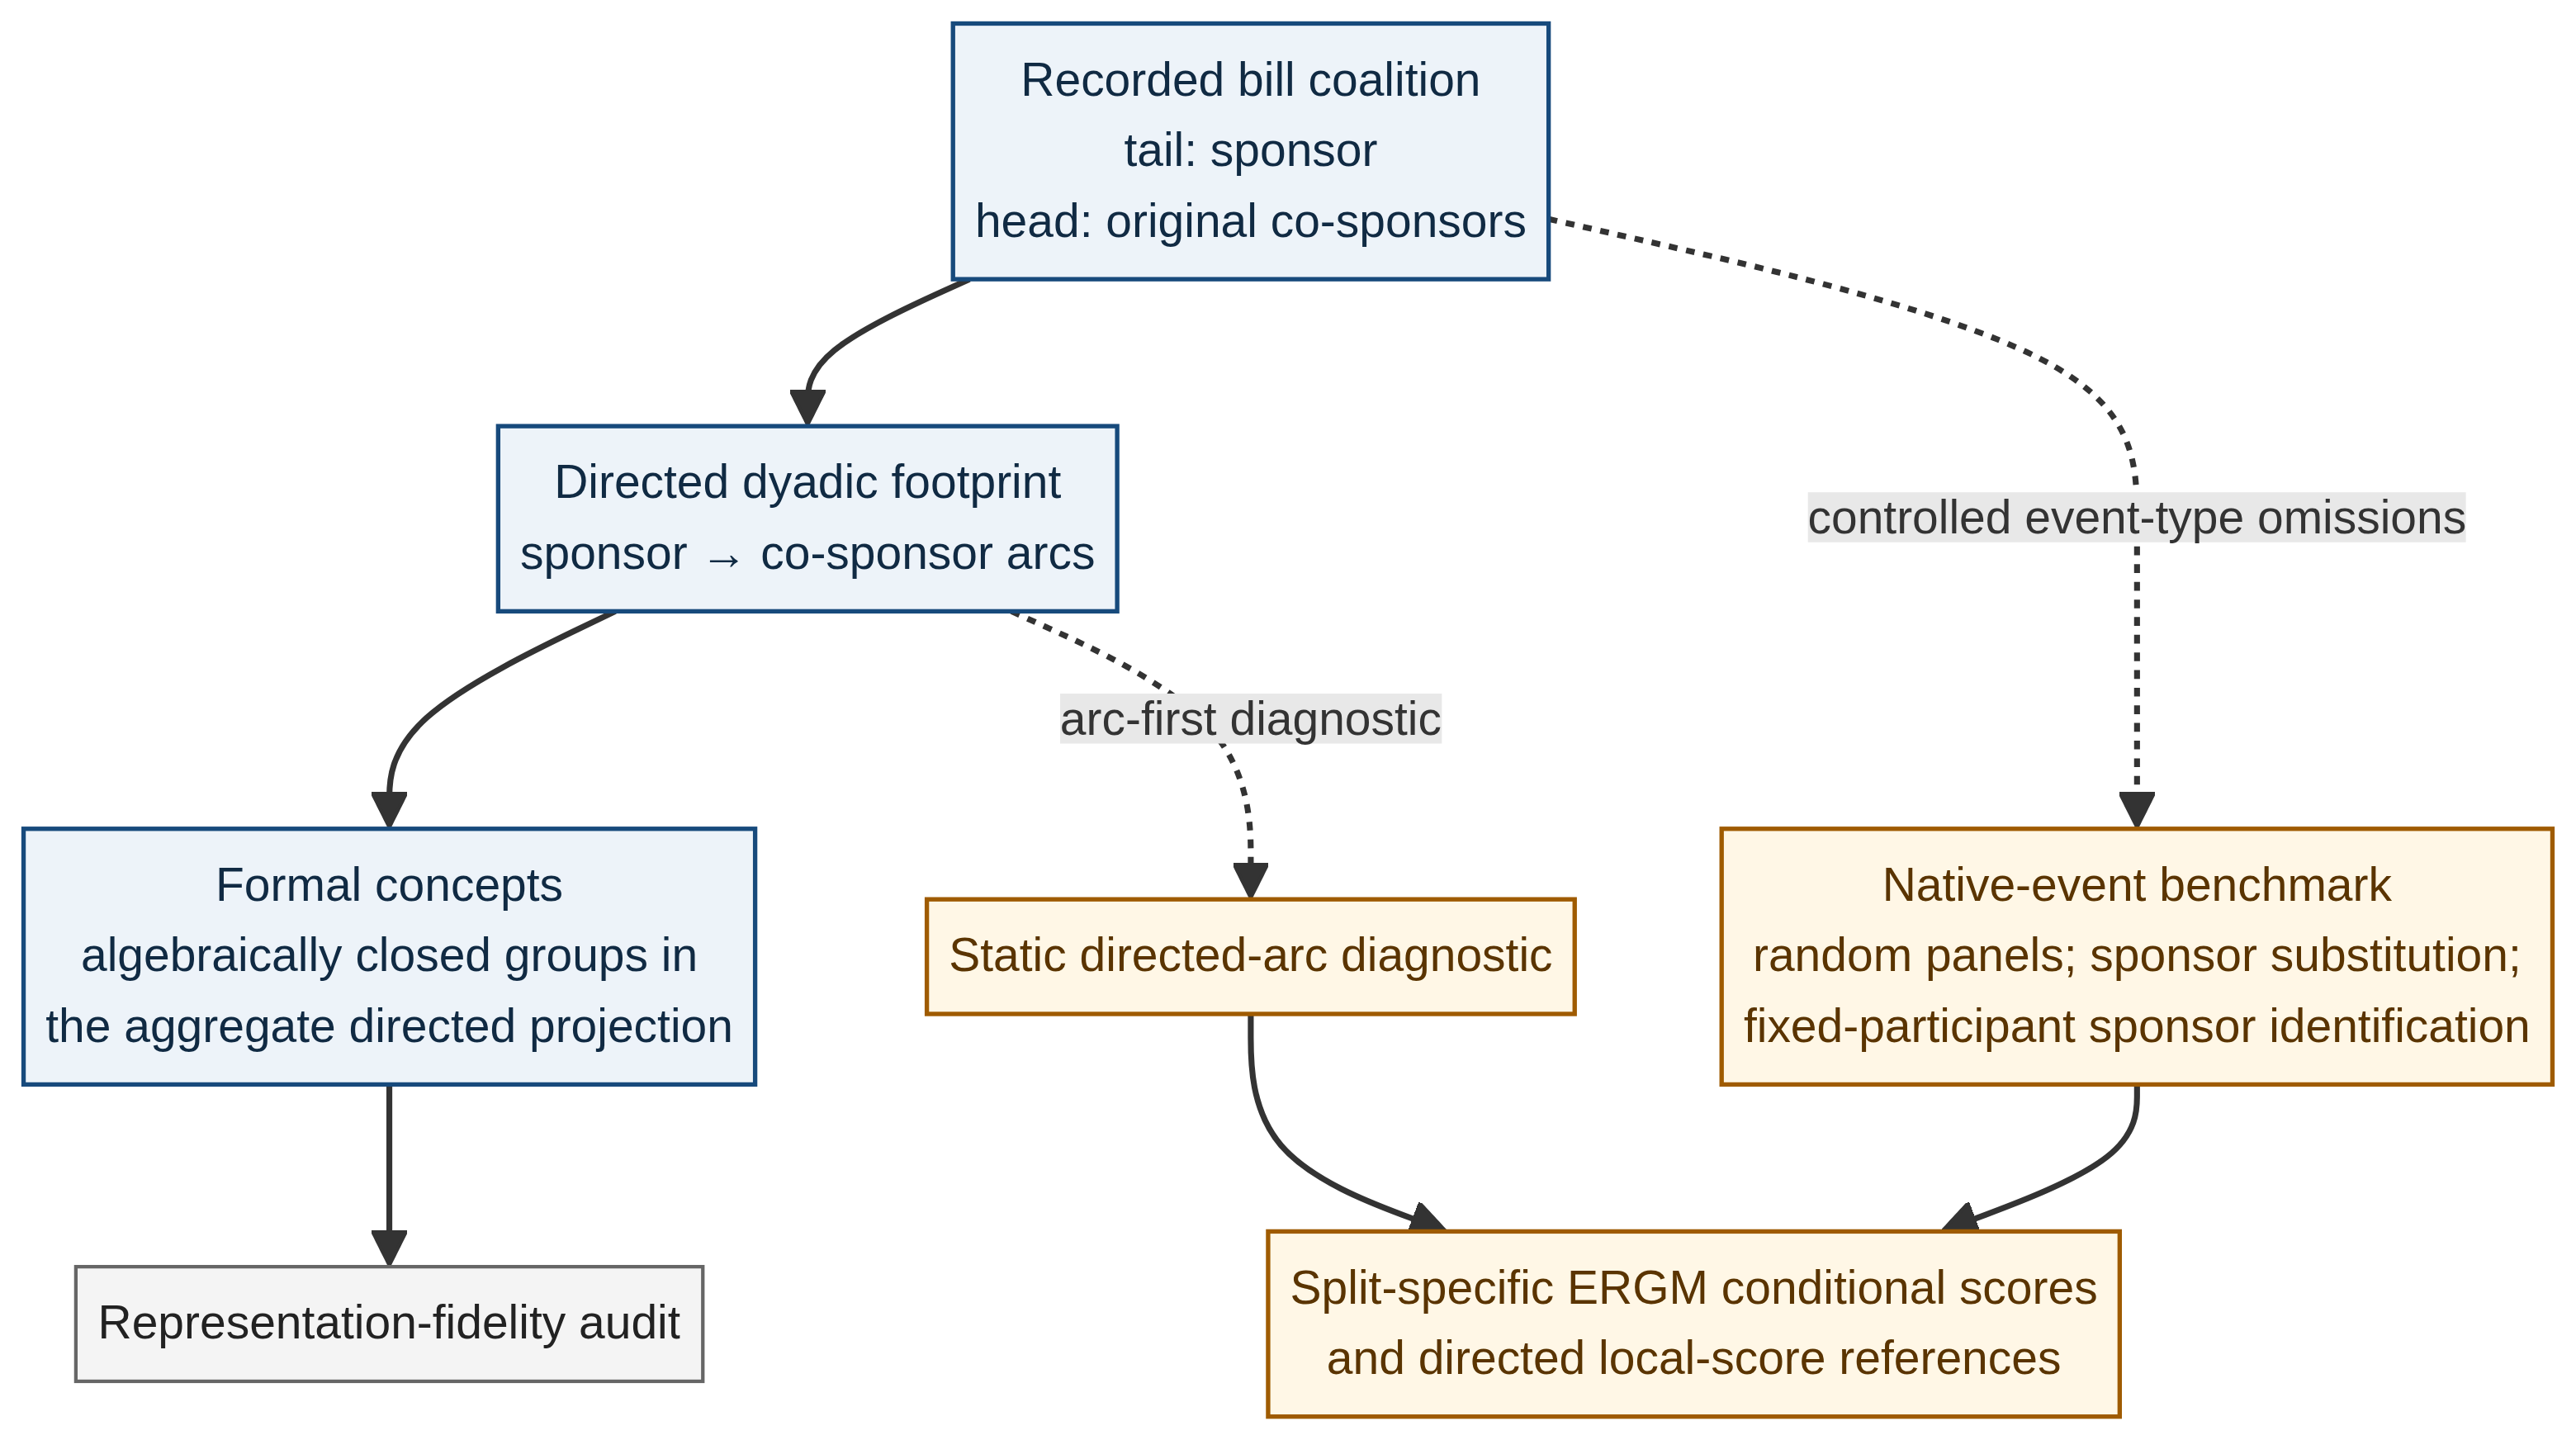
\includegraphics[width=0.98\textwidth]{figures/fig1_senate_target_ladder.png}
\caption{Target ladder for the Senate benchmark. The event-first benchmark evaluates recorded bill coalitions; the static arc diagnostic evaluates the projection; formal concepts are an algebraically derived representation whose correspondence with recorded coalitions is measured rather than assumed.}
\label{fig:target-ladder}
\end{figure}

\subsection{Directed local statistics and ERGM conditionals}

For an ordered dyad $(i,j)$, write $N_Y^+(i)=\{k:Y_{ik}=1\}$ and $N_Y^-(i)=\{k:Y_{ki}=1\}$. The directed out--in common-neighbour count is
\begin{equation}
 c_{ij}^{OI}(Y)=\sum_{k\in V\setminus\{i,j\}}Y_{ik}Y_{kj}
 =|N_Y^+(i)\cap N_Y^-(j)|.
 \label{eq:oi}
\end{equation}
We also evaluate out--out and in--in overlaps,
\begin{equation}
 c_{ij}^{OO}=|N_Y^+(i)\cap N_Y^+(j)|,
 \qquad
 c_{ij}^{II}=|N_Y^-(i)\cap N_Y^-(j)|,
 \label{eq:directed-overlaps}
\end{equation}
and their sum $c_{ij}^{\mathrm{total}}=c_{ij}^{OI}+c_{ij}^{OO}+c_{ij}^{II}$. The components have different directional meanings: OI counts a directed two-path from $i$ to $j$, OO counts shared targets, and II counts shared sources. Retaining them separately prevents a directed score from becoming an undirected neighbourhood overlap with relabelled endpoints.

For degree-discounted variants, let $d_i^+=|N_Y^+(i)|$, $d_i^-=|N_Y^-(i)|$, and $w(d)=1/\log d$ for $d>1$ and zero otherwise. The implemented directed Adamic--Adar components are
\begin{align}
 a_{ij}^{OI}&=\sum_{k\in N_Y^+(i)\cap N_Y^-(j)}w(d_k^++d_k^-),\\
 a_{ij}^{OO}&=\sum_{k\in N_Y^+(i)\cap N_Y^+(j)}w(d_k^-),\\
 a_{ij}^{II}&=\sum_{k\in N_Y^-(i)\cap N_Y^-(j)}w(d_k^+),
 \qquad a_{ij}^{\mathrm{total}}=a_{ij}^{OI}+a_{ij}^{OO}+a_{ij}^{II}.
 \label{eq:directed-aa}
\end{align}
An OI intermediary is discounted by total directed activity, a shared target by incoming popularity, and a shared source by outgoing broadcast activity. We further evaluate reverse-arc support $r_{ij}=Y_{ji}$ and degree product $b_{ij}=d_i^+d_j^-$. The first is direct reciprocity; the second combines sponsor-side activity and co-sponsor-side popularity without requiring a common neighbour.

For any dyadic statistic $x_{ij}$, the mean-lifted event score is
\begin{equation}
 \bar{x}(T,H)=\frac{1}{|T||H|}\sum_{i\in T}\sum_{j\in H}x_{ij}.
 \label{eq:local-score-lift}
\end{equation}
This uses only the observed split projection. It is an uncalibrated ranking statistic rather than a group-event likelihood. The same footprint convention makes local and ERGM scores comparable inside a declared candidate panel, while retaining their different interpretations.

For an ERGM with sufficient statistics $g(Y)$,
\begin{equation}
 \Pr_{\theta}(Y=y)=\frac{\exp\{\theta^{\top}g(y)\}}{\kappa(\theta)},
 \label{eq:ergm}
\end{equation}
the exact full-conditional probability of one tie, given every other tie, is
\begin{equation}
 \Pr_{\theta}(Y_{ij}=1\mid Y_{-ij})=
 \operatorname{logit}^{-1}\{\theta^{\top}\Delta_{ij}g(Y)\},
 \qquad
 \Delta_{ij}g(Y)=g(Y^{+ij})-g(Y^{-ij}).
 \label{eq:ergm-conditional}
\end{equation}
For a directed transitive-triple term, the change statistic is $c_{ij}^{OI}(Y)$. A one-covariate conditional logit with positive transitive-triple coefficient therefore orders dyads in the same direction as the directed common-neighbour statistic. We fit this restricted check independently on every Senate training projection; it verifies the sign and rank relation empirically without treating it as a complete ERGM.

The benchmark ladder distinguishes density, mutuality, degree heterogeneity, and directed closure. Let $E(Y)=\sum_{i\ne j}Y_{ij}$ and $R(Y)=\sum_{i<j}Y_{ij}Y_{ji}$ denote edge and mutual-dyad counts. For decay $\alpha>0$, define $f_\alpha(k)=e^\alpha[1-(1-e^{-\alpha})^k]$, with $f_\alpha(0)=0$. The geometrically weighted outgoing- and incoming-degree statistics are $G^+(Y)=\sum_i f_\alpha(d_i^+)$ and $G^-(Y)=\sum_i f_\alpha(d_i^-)$. Their diminishing increments represent degree structure without duplicating the linear edge count.

For $Q\in\{OI,OO,II\}$, the corresponding directed shared-partner statistic is
\begin{equation}
 W_Q(Y)=\sum_{i\ne j}Y_{ij}f_\beta\left(c_{ij}^{Q}(Y)\right),
 \label{eq:shared-partner}
\end{equation}
where the count is evaluated on an existing arc and the toggle can affect the partner counts of other arcs. $W_{OI}$ is outgoing two-path closure, while $W_{OO}$ and $W_{II}$ represent shared-target and shared-source closure. The cyclic term counts directed cycles $i\to j\to k\to i$. With the fixed decays $\alpha=\beta=0.5$, the nested specifications are
\begin{align}
 \mathrm{M0}:&\quad E, & \mathrm{M1}:&\quad E,R,\\
 \mathrm{M2}:&\quad E,R,G^+,G^-, & \mathrm{M3}:&\quad \mathrm{M2}+W_{OI},\\
 \mathrm{M4}:&\quad \mathrm{M3}+W_{OO}+W_{II}, & \mathrm{M4c}:&\quad \mathrm{M4}+g_{\mathrm{cyclic}}.
 \label{eq:ergm-ladder}
\end{align}
The names identify nested score specifications, not separate causal effects. For example, the M4c--M3 difference changes multiple shared-partner terms and cyclic structure together. Every model is fitted by maximum pseudolikelihood estimation (MPLE) on the observed projection of each mask. MPLE makes the conditional-score comparison computationally feasible, but it differs from likelihood-based ERGM inference and from simulation-based joint event prediction \citep{vanDuijnEtAl2009,hunterEtAl2008}.

Let $p_{ij}$ denote the split-specific ERGM conditional score in \eqref{eq:ergm-conditional}. For a candidate footprint $F=\phi(T,H)$, we report
\begin{align}
 L_1(F)&=|F|^{-1}\sum_{(i,j)\in F}p_{ij},\\
 L_{1g}(F)&=\exp\left\{|F|^{-1}\sum_{(i,j)\in F}\log p_{ij}\right\},\\
 L_2(F)&=\prod_{(i,j)\in F}p_{ij}.
 \label{eq:footprint-scores}
\end{align}
The main ERGM ranking score is $L_{1g}$, the size-normalized geometric mean. These are factorized products or summaries of single-dyad conditionals, each conditioned on the training network. They are discriminative footprint scores, not the joint probability that the complete ordered coalition occurred. This distinction is essential: the likelihood in \eqref{eq:ergm} is a network model, whereas the event benchmark asks the score to discriminate observed and constructed coalition candidates.

\section{Data and benchmark design}\label{sec:data-methods}

\subsection{Senate Bill Status event construction}\label{sec:senate-data}

The political application uses the completed 118th Congress (3 January 2023--3 January 2025) and Senate bills (S.) only. The official GPO Bill Status XML archive supplies stable bill identifiers, introduction information, a sponsor Bioguide identifier, and a co-sponsor record with \texttt{bioguideId}, \texttt{isOriginalCosponsor}, sponsorship date, and withdrawal information \citep{gpoBillStatus,congressGovBillStatus}. One native record is one S. bill. Its tail is the unique recorded sponsor; its head is the set of distinct co-sponsors with \texttt{isOriginalCosponsor = True}. The target preserves an original co-sponsor who subsequently withdrew because it represents membership at introduction, not a later endpoint of the bill's co-sponsorship history.

The archive contains 5,649 bill-status XML records. Exactly 4,374 measures have a nonempty original-co-sponsor head; 1,275 have none and are reported rather than silently absorbed into a singleton-link target. No record was excluded for a missing or non-single sponsor, no duplicate original-co-sponsor row was found, and six original co-sponsors with a later withdrawal remain in the introduction-time event. Table~\ref{tab:senate-data} gives the resulting primary accounting.

\begin{table}[tbp]
\centering
\small
\caption{Senate co-sponsorship record construction and fixed actor universe.}
\label{tab:senate-data}
\begin{tabular}{p{0.50\textwidth}p{0.40\textwidth}}
\toprule
Quantity & Value \\
\midrule
Bill Status XML records (118th Congress, S. bills) & 5,649 \\
Measures with nonempty original-co-sponsor head & 4,374 \\
Measures with zero original co-sponsors & 1,275 \\
Distinct Senate persons in primary universe & 105 \\
Directed sponsor-to-co-sponsor arcs & 5,619 \\
Primary event target & one sponsor $\to$ up to ten original co-sponsors \\
Missingness grid & 30 MCAR + 30 activity-biased MNAR-out masks \\
\bottomrule
\end{tabular}
\par\vspace{2pt}\footnotesize A record is an S. bill with its sole recorded sponsor as tail and its original co-sponsors as head. Later withdrawals remain in the introduction-time membership target.
\end{table}


The Senate has 100 seats but a two-year Congress can include replacements and vacancies. We compared a 100-person reference-date roster with a universe of all distinct persons whose Senate term overlaps the Congress. The former loses 204 valid nonempty-head events. The latter has 105 persons and retains every valid event without merging people by seat. We therefore use the 105-person universe throughout the primary benchmark. The comparison in Appendix~\ref{app:senate-audit} is a measurement decision rather than a convenience: a seat-merging rule would manufacture continuity between different actors.

\subsection{Cap selection before primary masking}\label{sec:cap-selection}

The target has a singleton sponsor tail but potentially large co-sponsor heads. A common cap of three would remove a non-random subset of Senate bills. We therefore evaluated $|H|\leq1,2,3,5,10$ with the fixed 105-person universe before the full experiment. Each cap profile reports retention of records and ordered types, projection coverage, candidate capacity, cap-first formal-concept feasibility, and a small end-to-end score pilot. The primary cap is $|T|\leq1,|H|\leq10$, with no truncation: bills above the cap are outside the primary target rather than artificially shortened.

The choice preserves 90.4\% of valid bill records and 88.5\% of distinct ordered types. It is also the first evaluated cap at which the bounded formal-concept target is nonempty (16 concepts) and all three M0/M4c pilot fits and conditional-score runs complete. Appendix~\ref{app:senate-audit} provides the full cap audit. An independently seeded $|H|\leq3$ sensitivity uses the same event-first design and is reported separately; it does not revise the primary cap after observing primary results.

\subsection{Event-first missingness mechanisms}\label{sec:masking}

Let $\mathcal{E}_{c}$ be the cap-eligible set of distinct native event types, and let $q=0.30$ be the nominal withheld-type rate. For a mask replicate $r$, the MCAR mechanism samples exactly $\lfloor q|\mathcal{E}_{c}|\rfloor$ types uniformly without replacement. The observed event set and projection are
\begin{equation}
 \mathcal{E}^{(r)}_{\mathrm{obs}}=\mathcal{E}_{c}\setminus\mathcal{M}^{(r)},
 \qquad Y^{(r)}=Y\!\left(\mathcal{E}^{(r)}_{\mathrm{obs}}\right),
 \label{eq:event-mask}
\end{equation}
where $\mathcal{M}^{(r)}$ is the set of held-out types. Every occurrence of a selected type is removed together. This avoids direct target leakage through a repeated identical tail/head pair.

MNAR-out is an explicitly oracle, activity-biased stress test. Let $a_s(e)$ be the full cap-eligible outgoing recipient incidence of the singleton sponsor of event type $e$. A type is independently withheld with probability
\begin{equation}
 \pi_e=\min\{1,\lambda a_s(e)\},
 \qquad \frac{1}{|\mathcal{E}_c|}\sum_{e\in\mathcal{E}_c}\pi_e=q,
 \label{eq:mnar}
\end{equation}
where $\lambda$ is solved numerically. The realised rate can differ from $q$. The mechanism is useful precisely because its dependence on complete data is explicit; it is not a diagnosis of the archival process. We generate 30 independently seeded MCAR masks and 30 MNAR-out masks. Appendix~\ref{app:mask-diagnostics} reports realised rates, arc loss, and the proportion of withheld coalition types whose complete dyadic footprint survives through other observed bills.

A surviving footprint is informative rather than leakage. Equation~\eqref{eq:projection} implies that an arc of a held-out coalition may remain in $Y^{(r)}$ if another observed bill uses the same sponsor--co-sponsor dyad. The benchmark consequently records an already-observed-footprint baseline rather than treating all positive types as equally novel in dyadic terms.

\subsection{Candidate panels and political role tests}\label{sec:panels}

Each evaluation panel is built from the training split $\mathcal{E}^{(r)}_{\mathrm{obs}}$ and its projection only. The random panel pairs a held-out positive event $e=(T,H)$ with an arity-matched admissible non-event $e'$ under the same singleton-sponsor grammar. It asks whether a score can rank the omitted coalition over randomly constructed alternatives with the same tail and head arities.

The Senate hard panel is deliberately more demanding. For a held-out bill with participant set $P=T\cup H$, an eligible original co-sponsor $h\in H$ becomes the substitute sponsor and the original sponsor enters the head:
\begin{equation}
 e^{(h)}=(\{h\},(H\setminus\{h\})\cup T).
 \label{eq:sponsor-substitution}
\end{equation}
The participant set, head size, and one-sponsor grammar are fixed. A literal tail/head reversal would convert a valid one-sponsor-to-many-co-sponsor event into an implausible many-sponsor event, so it is not the political orientation task.

The role-assignment panel is exhaustive within the same grammar. Conditional on $P$ and $|H|$, every $p\in P$ defines a candidate $(\{p\},P\setminus\{p\})$ compatible with a single sponsor. Top-1 accuracy is the proportion of bills for which the observed sponsor has the highest score; mean reciprocal rank (MRR) uses the rank of the observed sponsor among all compatible assignments. This asks a more interpretable political question than random nonedge ranking: who is identified as the bill's agenda-setting sponsor when every candidate has the same participants and arity?

\subsection{Performance measures and paired uncertainty}\label{sec:evaluation}

PR-AUC is the principal ranking measure because prevalence in each constructed panel is set by design; ROC-AUC is reported as a threshold-free companion \citep{saitoRehmsmeier2015}. For ranked labels $z$ and scores $s$, PR-AUC summarizes the precision--recall curve after positives and negatives have been defined by the panel, whereas ROC-AUC summarizes the true-positive versus false-positive ordering. Neither score is a calibrated event probability. The role-assignment task instead reports top-1 accuracy and MRR because its candidate sets are multiclass partitions rather than balanced binary panels.

For a comparison method $A$ versus reference $B$, let $D_r=m_{A,r}-m_{B,r}$ be the metric difference on matched mask $r$. We report $\bar D=30^{-1}\sum_rD_r$, a percentile bootstrap interval from 10,000 resamples of the 30 complete masks, and a two-sided sign-flip randomization $p$-value from 20,000 sign permutations. The resampling unit is the whole mask so that all events, candidates, and scores created from a split stay together. These intervals describe split-to-split variation inside the fixed constructed Senate network; they do not establish population uncertainty over legislatures or over historical periods \citep{efronTibshirani1994}.

\subsection{Reproducibility, privacy, and non-political scope checks}\label{sec:scope}

The Senate source is public, but reproducibility does not require release of every intermediate object. The repository contains acquisition and parsing code, checksums, data-policy records, aggregate outputs, table and figure generators, and the manuscript sources. It excludes raw XML copies, processed event rows, actor-level candidate panels, fitted objects, and prediction-level records. The Enron branch remains subject to a stricter privacy boundary: it never publishes e-mail content or addresses.

The same event-first pipeline is retained for an Enron strict custodian core and a reconstructed MathOverflow core. They test whether the benchmark architecture can be executed on distinct directed event records. They are not political cases and do not drive the framing, target choice, or conclusion of this manuscript. Their aggregate results appear only as scope checks in Appendix~\ref{app:scope-checks}.

\section{Results}\label{sec:results}

\subsection{Projection-derived concepts differ from recorded coalitions}\label{sec:concept-results}

At the selected cap, the Senate projection yields 16 formal concepts and 3,209 cap-eligible recorded bill types. Their ordered tail/head intersection is exactly zero. The concepts cover 251 directed arcs, whereas the recorded bill types cover 4,290; their footprint Jaccard similarity is 0.048 (Table~\ref{tab:senate-fidelity}; Figure~\ref{fig:senate-fidelity}). The aggregate projection therefore retains a small closure structure that is neither a reconstruction nor a partition of recorded bill coalitions.

This result is not a statement that formal concepts are uninformative. They may describe recurring maximal co-sponsorship patterns in the projected relation. It is instead a statement about identification: an analyst who extracts a concept from $Y$ must name it as a projection-derived structure. The recorded bill coalition remains a distinct empirical object tied to a bill identifier and an introduction-time membership rule.

\begin{table}[tbp]
\centering
\small
\caption{Cap-dependent formal-concept fidelity versus recorded Senate bill coalitions.}
\label{tab:senate-fidelity}
\begin{tabular}{lrrrr}
\toprule
Head cap & concepts & bill types & exact matches & footprint $J$ \\
\midrule
$|H|\leq10$ (primary) & 16 & 3,209 & 0 & 0.048 \\
$|H|\leq15$ (alternative) & 474 & 3,398 & 0 & 0.610 \\
\bottomrule
\end{tabular}
\par\vspace{2pt}\footnotesize Both enumerations use the aggregate projection and $|T|\leq3$. Exact agreement requires equality of ordered tail and head sets; footprint $J$ compares unions of directed arcs under the stated cap.
\end{table}

\begin{figure}[tbp]
\centering
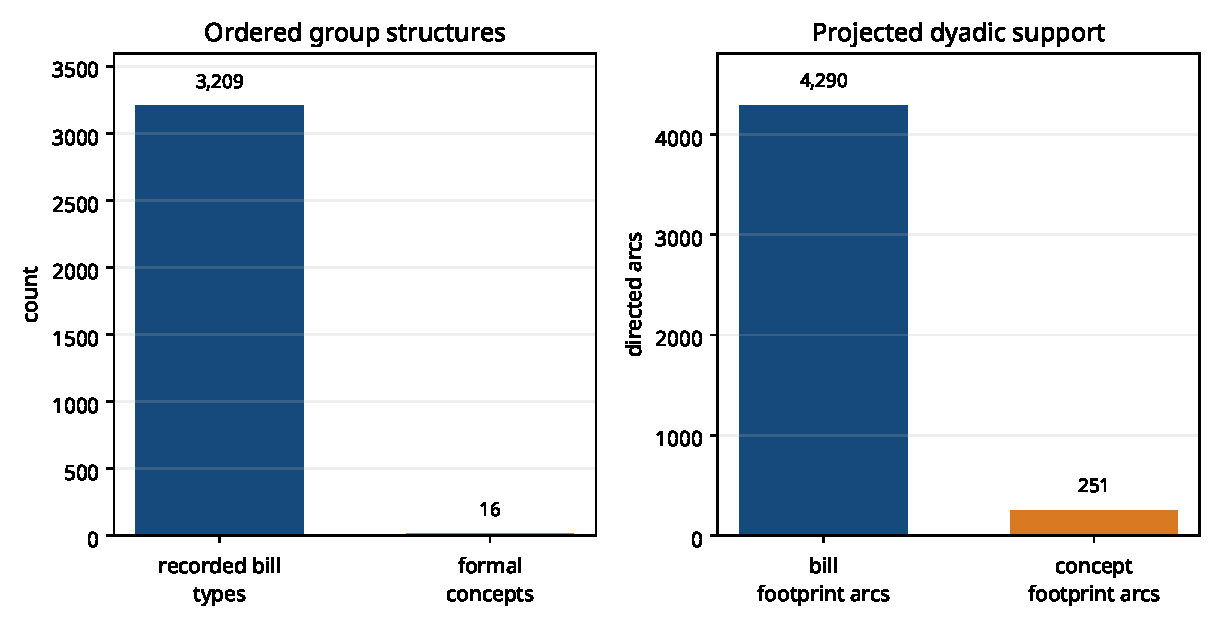
\includegraphics[width=0.96\textwidth]{figures/fig3_senate_concept_event_fidelity.pdf}
\vspace{3mm}
\caption{Recorded Senate bill coalition types and their directed footprints versus formal concepts generated from the aggregate projection. The difference in scale and the zero exact ordered matches show that closure-derived concepts are not a reconstruction of bill coalitions.}
\label{fig:senate-fidelity}
\end{figure}

\subsection{Conditional ERGM scores exceed density but not the strongest local reference}\label{sec:footprint-results}

Table~\ref{tab:senate-performance} and Figure~\ref{fig:senate-performance} compare the declared local reference with M4c conditional $L_{1g}$. On random panels, M4c reaches PR-AUC 0.704 under MCAR and 0.749 under MNAR-out. Relative to M0's density-only score, the paired PR-AUC increase is 0.204 (95\% CI [0.200, 0.209]) under MCAR and 0.249 ([0.243, 0.254]) under MNAR-out, with the simulation-limited sign-flip $p=0.00005$ in each case. Conditional structural terms therefore provide substantial random-panel discrimination beyond density.

The density comparison is an insufficient competitive benchmark. Directed Adamic--Adar total reaches PR-AUC 0.743 and 0.793 under MCAR and MNAR-out on the random panel, exceeding M4c by 0.038 ([0.035, 0.042]) and 0.044 ([0.039, 0.050]). The result is not caused by an unexamined model-level choice: Table~\ref{tab:ergm-ladder} gives the full M0--M4c ladder. M2 has random-panel PR-AUC 0.703 and 0.732, while the added shared-partner terms in M3--M4c provide little additional random-panel gain in this construction. The appropriate conclusion is narrow: the split-specific conditional M4c footprint score is not the highest ranking score among the declared transparent local references for these Senate candidate panels.

On grammar-preserving sponsor substitution, degree product also outperforms M4c. The paired M4c-minus-degree-product PR-AUC differences are $-0.108$ (95\% CI [$-0.114,-0.103$]) under MCAR and $-0.081$ ([$-0.089,-0.074$]) under MNAR-out. This harder panel is politically meaningful because it asks the score to distinguish an observed coalition from a coalition with the same participants but a different sponsor. The pattern shows why a density baseline cannot stand in for the best available directed local comparator.

\begin{table}[tbp]
\centering
\small
\caption{Primary Senate native-event footprint recovery across matched masks.}
\label{tab:senate-performance}
\begin{tabular}{llllrr}
\toprule
Mask & panel & score & score class & PR-AUC & ROC-AUC \\
\midrule
MCAR & random & AA-total & 0.743 & 0.743 \\
MCAR & random & M4c conditional & 0.704 & 0.722 \\
MCAR & sponsor substitution & degree product & 0.580 & 0.590 \\
MCAR & sponsor substitution & M4c conditional & 0.472 & 0.463 \\
MNAR-out & random & AA-total & 0.793 & 0.811 \\
MNAR-out & random & M4c conditional & 0.749 & 0.772 \\
MNAR-out & sponsor substitution & degree product & 0.567 & 0.590 \\
MNAR-out & sponsor substitution & M4c conditional & 0.485 & 0.489 \\
\bottomrule
\end{tabular}
\par\vspace{2pt}\footnotesize Entries are means over 30 matched masks. M4c uses split-specific MPLE estimates and the factorized conditional footprint score $L_{1g}$; it is not a joint coalition probability.
\end{table}

\begin{table}[tbp]
\centering
\small
\caption{Matched-mask difference between M4c $L_{1g}$ and the declared local reference.}
\label{tab:senate-contrasts}
\begin{tabular}{lllrrr}
\toprule
Mask & panel & metric & difference & 95\% CI & sign-flip $p$ \\
\midrule
MCAR & random & PR-AUC & -0.041 & [-0.045, -0.037] & $\leq0.00005$ \\
MCAR & random & ROC-AUC & -0.021 & [-0.024, -0.018] & $\leq0.00005$ \\
MNAR-out & random & PR-AUC & -0.045 & [-0.050, -0.040] & $\leq0.00005$ \\
MNAR-out & random & ROC-AUC & -0.040 & [-0.044, -0.037] & $\leq0.00005$ \\
MCAR & sponsor substitution & PR-AUC & -0.108 & [-0.114, -0.103] & $\leq0.00005$ \\
MCAR & sponsor substitution & ROC-AUC & -0.127 & [-0.132, -0.122] & $\leq0.00005$ \\
MNAR-out & sponsor substitution & PR-AUC & -0.081 & [-0.089, -0.074] & $\leq0.00005$ \\
MNAR-out & sponsor substitution & ROC-AUC & -0.102 & [-0.110, -0.093] & $\leq0.00005$ \\
\bottomrule
\end{tabular}
\par\vspace{2pt}\footnotesize Difference = M4c $L_{1g}$ minus AA-total on random panels and minus degree product on sponsor-substitution panels. Intervals resample whole masks within the fixed Senate network.
\end{table}

\begin{figure}[tbp]
\centering
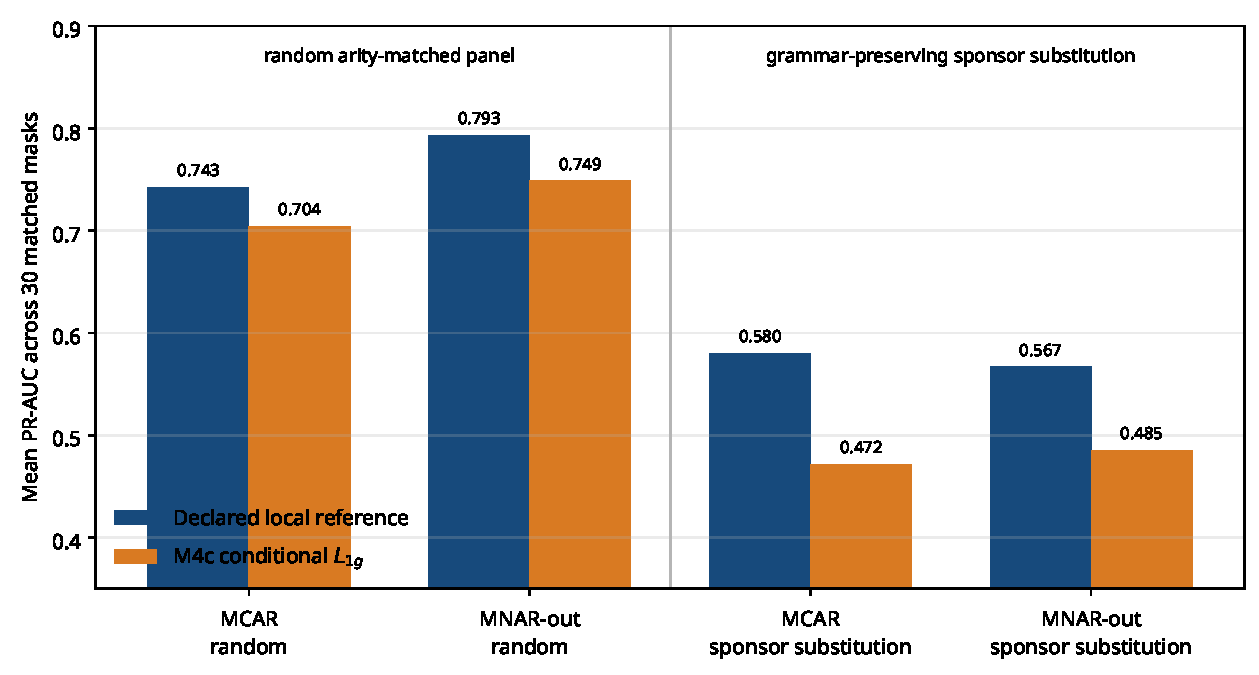
\includegraphics[width=0.96\textwidth]{figures/fig2_senate_primary_pr_auc.pdf}
\vspace{2mm}
\caption{Mean PR-AUC across 30 matched masks for the Senate native-event footprint target. The random and sponsor-substitution panels ask different questions; the latter preserves the one-sponsor political event grammar.}
\label{fig:senate-performance}
\end{figure}

\subsection{Sponsor identification is a distinct political role task}\label{sec:role-results}

The role-assignment task conditions on the actors and arity of each bill coalition and asks which compatible partition places the recorded sponsor in the tail. The local AA-OI reference yields top-1 accuracy 0.429 under MCAR and 0.402 under MNAR-out, with MRR 0.649 and 0.633. M4c produces top-1 accuracy 0.304 and 0.311, with MRR 0.562 and 0.567 (Table~\ref{tab:senate-role}). These are not prevalence-weighted binary classification measures: each bill is evaluated against all compatible one-sponsor partitions.

The comparison makes the role content of direction visible. A score can successfully rank a withheld footprint above random coalitions while remaining less effective at identifying who occupies the sponsor role when the participant set is fixed. In substantive terms, the latter task is closer to the leadership and agenda-setting distinction that motivates directed co-sponsorship data. It should therefore be presented alongside, rather than inferred from, random-panel performance.

\begin{table}[tbp]
\centering
\small
\caption{Sponsor identification with participants and arities held fixed.}
\label{tab:senate-role}
\begin{tabular}{lrrr}
\toprule
Mask & score & top-1 accuracy & MRR \\
\midrule
MCAR & AA-OI & 0.429 & 0.649 \\
MCAR & M4c conditional & 0.304 & 0.562 \\
MCAR & uniform chance & 0.330 & 0.581 \\
MCAR & M5 political conditional & 0.316 & 0.573 \\
MCAR & M6 sender-effect conditional & 0.325 & 0.579 \\
MNAR-out & AA-OI & 0.402 & 0.633 \\
MNAR-out & M4c conditional & 0.311 & 0.567 \\
MNAR-out & uniform chance & 0.319 & 0.569 \\
MNAR-out & M5 political conditional & 0.320 & 0.575 \\
MNAR-out & M6 sender-effect conditional & 0.328 & 0.579 \\
\bottomrule
\end{tabular}
\par\vspace{2pt}\footnotesize Each held-out bill is evaluated against every compatible sponsor/co-sponsor partition. Local rows are event-weighted over observed arities; chance is $1/(|H|+1)$ for top-1. ERGM rows use factorized conditional $L_{1g}$ scores.
\end{table}


\subsection{Cap, directed-link, and non-political checks}\label{sec:supplementary-results}

The independent $|H|\leq3$ rerun retains the same actor universe, event-first masking design, and 30 masks. Relative to density, M4c $L_{1g}$ improves random-panel PR-AUC by 0.191 (95\% CI [0.187, 0.196]) under MCAR and 0.218 ([0.213, 0.223]) under MNAR-out (Table~\ref{tab:senate-cap-sensitivity}). The directional conclusion against density therefore persists at the smaller cap, although the cap changes the event target and substantially reduces retention. This is why the cap-three analysis is a sensitivity, not a substitute for the cap-ten primary target.

A one-covariate transitive-triple logistic check was fitted to every Senate training projection. In all 60 splits, the directed transitive-triple coefficient is positive and the conditional rank direction agrees with the directed common-neighbour statistic. The bounded static arc diagnostic and the full split summary are reported in Appendix~\ref{app:directed-link}. These results support the directed-link component of the benchmark, while remaining separate from native coalition recovery.

The Enron and MathOverflow scope checks preserve the event-first framework but are not used to generalize a political conclusion. They demonstrate that the distinction between a recorded event, its footprint, and a derived group is not a peculiarity of the Senate source. Appendix~\ref{app:scope-checks} reports their aggregate random-panel results and retains their distinct provenance and reconstruction boundaries.

\begin{table}[tbp]
\centering
\small
\caption{Cap-three sensitivity: paired M4c $L_{1g}$ versus density-only random-panel PR-AUC.}
\label{tab:senate-cap-sensitivity}
\begin{tabular}{llrr}
\toprule
Cap & mask & difference & 95\% CI \\
\midrule
$|H|\leq3$ & MCAR & 0.177 & [0.172, 0.183] \\
$|H|\leq3$ & MNAR-out & 0.210 & [0.204, 0.215] \\
\bottomrule
\end{tabular}
\par\vspace{2pt}\footnotesize The primary cap is $|H|\leq10$; this independent cap-three rerun preserves the fixed Senate actor universe, event-first masking design, and 30 masks per mechanism.
\end{table}


\section{Discussion}\label{sec:discussion}

The Senate application makes explicit a distinction that can otherwise remain hidden in political-network workflows. A sponsor-to-co-sponsor projection is a useful directed network, but it is not a record of coalition membership. The cap-first concept audit makes the distinction empirical: projection-derived formal concepts share limited dyadic support with recorded coalition types and have zero exact ordered matches. The result cautions against equating a structurally closed group in an aggregate co-sponsorship network with an original legislative coalition.

The benchmark also shows why political direction must be evaluated through a role-respecting candidate grammar. A literal reversal of a Senate bill would be an implausible many-sponsor event. Sponsor substitution and exhaustive fixed-participant role assignment instead preserve the political event grammar while asking whether the sponsor can be identified. In this setting, the local reference outperforms the M4c conditional score on sponsor substitution and role assignment, even though M4c materially exceeds density on random panels. The contrast is a result about the relationship among model, target, and candidate task, not a general ordering of ERGMs and local heuristics.

Three methodological implications follow. First, an event-level evaluation cannot be inferred from a static arc score, because the projection map in Proposition~1 discards event partition information. Second, a formal-concept evaluation answers a third question about closure in an aggregate relation; it should be audited against native records rather than treated as a proxy for them. Third, a conditional ERGM footprint score must be interpreted at its actual level of factorization. The score combines conditional tie support under an MPLE-fitted network model; it does not provide a simulated joint probability for a bill coalition.

The design also sets deliberate limits. MCAR and activity-biased MNAR-out are controlled stress tests, not assertions that the official archive is naturally MCAR or MNAR. Bootstrap intervals resample fixed-network masks and do not estimate cross-legislature uncertainty. The data construction covers Senate bills in one completed Congress and one explicit original-co-sponsor policy; it does not establish the same performance for House measures, other legislatures, treaties, or informal coalitions. Finally, the analysis does not conduct rolling-origin forecasting, STERGM estimation, relational hyperevent modelling, or neural hyperlink-prediction comparisons. Those questions require temporal targets, event hazards, and validation designs outside this paper's missingness-centred objective \citep{lernerLomi2023}.

The framework is nevertheless portable. Whenever a political record combines ordered roles with collective membership, analysts can state the native target, define its projection, audit derived group structures, and construct role-valid alternatives before comparing models. The next scientific step is an externally validated comparison across political record systems, with event semantics and actor identities audited separately. For the present legislative record, the main lesson is clear: projection can preserve dyadic support while changing the prediction target, and ERGM evaluation must be tied to the target and candidate grammar that the political question actually specifies.

\appendix

\section{Senate source, actor, and cap audits}\label{app:senate-audit}

\subsection{Source contract and event parsing}

The primary archive is the GPO Bill Status XML directory for 118th-Congress Senate bills. The acquisition script stores the official directory URL, listing checksum, file-tree checksum, record count, and access time. It retrieves the XML snapshot rather than scraping rendered pages. The event parser requires exactly one sponsor identifier and reads only co-sponsor entries explicitly marked original. It deduplicates repeated original-co-sponsor identifiers within a bill, preserves the introduction-time member even when a later withdrawal is present, and excludes empty-head measures only from the nonempty-head hyperlink target. This construction is deliberately narrower than a general longitudinal account of co-sponsorship: it defines a fixed introduction-time group event appropriate for the benchmark.

The raw source is public, but the repository omits raw XML and processed event rows. The omission is a reproducibility design choice, not an obstacle to re-running the pipeline: the manifest identifies the official source and checksums, while the scripts reconstruct the event records. The same policy avoids publishing actor-level prediction candidates or fitted-score rows that are unnecessary for the aggregate results.

\begin{table}[tbp]
\centering
\small
\caption{Actor-universe audit before the primary Senate benchmark.}
\label{tab:actor-universe-audit}
\begin{tabular}{p{0.40\textwidth}rrrr}
\toprule
Policy & persons & retained bills & retention & projected arcs \\
\midrule
100 persons serving on 1 January 2024 & 100 & 4,170 & 95.3\% & 5,209 \\
all persons serving during the 118th Congress & 105 & 4,374 & 100.0\% & 5,619 \\
\bottomrule
\end{tabular}
\par\vspace{2pt}\footnotesize The selected policy retains every valid bill with a nonempty original-co-sponsor head and never merges distinct people by Senate seat.
\end{table}


\subsection{Why the actor policy is substantive}

A reference-date roster gives a superficially attractive 100-person network. It would, however, remove valid events involving senators whose service began or ended during the Congress. The all-serving-persons policy yields 105 actors, retains 100\% of valid nonempty-head bills, and does not merge people who occupied the same seat at different times. The fixed actor universe is used in every cap profile, split, candidate panel, and ERGM fit. Consequently, differences between the primary and cap-three analyses arise from the head cap rather than a changing set of political actors.

\subsection{Cap-first audit}

The cap controls the definition of the native event target. The audit evaluates retention and candidate feasibility before the primary masks are drawn. At $|H|\leq3$, only 68.0\% of bill records and 61.8\% of distinct event types remain; no bounded formal concept is enumerated. At $|H|\leq10$, 90.4\% of records and 88.5\% of types remain, the concept target has 16 members, and sponsor-substitution and role-assignment panels are available. The higher cap was therefore chosen before the 30-mask study; it is applied to the native-event, footprint, and formal-concept branches alike.

\begin{table}[tbp]
\centering
\small
\caption{Cap-first Senate target audit across original-co-sponsor head limits.}
\label{tab:cap-audit}
\begin{tabular}{lrrrrrr}
\toprule
Head cap & bill retention & type retention & arcs & concepts & sponsor swaps & role events \\
\midrule
1 & 45.2\% & 35.1\% & 1,271 & 0 & 823 & 1,271 \\
2 & 55.9\% & 47.5\% & 1,785 & 0 & 1,271 & 1,722 \\
3 & 68.0\% & 61.8\% & 2,523 & 0 & 1,789 & 2,240 \\
5 & 78.1\% & 73.9\% & 3,221 & 0 & 2,228 & 2,679 \\
10 & 90.4\% & 88.5\% & 4,290 & 16 & 2,758 & 3,209 \\
\bottomrule
\end{tabular}
\par\vspace{2pt}\footnotesize All rows use the same 105-person universe. Concepts use the cap-first $|T|\leq3$ enumeration; the primary cap $|H|\leq10$ was selected before the 30-mask study.
\end{table}


\section{Masking and candidate diagnostics}\label{app:mask-diagnostics}

\subsection{Type-level rather than record-level omission}

The event-first design withholds a distinct ordered tail/head type. This prevents the same ordered group from appearing in both training and test data merely because it has more than one source record. The event record count may nevertheless differ from the type count because several bills can share the same sponsor and original-co-sponsor set. For each split, the implementation records both rates, the number of distinct projection arcs removed, and the fraction of held-out types whose entire footprint is already induced by other observed event types.

The realised MCAR type rate is essentially the requested 30\%. MNAR-out has a similar mean realised type rate by construction, but differs in record and projection-arc removal because selection depends on the sponsor's full-data activity. In both mechanisms, about two fifths of held-out types retain a complete observed footprint. This is precisely why native event recovery is different from static link recovery: the target can be absent while all of its constituent arcs are still present in the projection.

\begin{table}[tbp]
\centering
\small
\caption{Realised omission and footprint-survival rates across primary Senate masks.}
\label{tab:mask-realisation}
\begin{tabular}{lrrrrr}
\toprule
Mask & masks & type rate & record rate & arc-removal rate & surviving footprints \\
\midrule
MCAR & 30 & 29.98\% & 30.03\% & 18.00\% & 42.79\% \\
MNAR-out & 30 & 30.09\% & 30.37\% & 14.82\% & 44.60\% \\
\bottomrule
\end{tabular}
\par\vspace{2pt}\footnotesize A surviving footprint means every dyad of a held-out bill type remains induced by at least one distinct observed bill type; it is a representation feature, not target leakage.
\end{table}


\subsection{Panel validity}

All negative candidates are constructed after masking. A random negative must satisfy the singleton-tail grammar, match the positive head size, contain actors from the fixed universe, and not coincide with an observed native event type. A sponsor-substitution negative additionally preserves the positive participant set. The role-assignment panel enumerates candidate singleton tails inside that set. These constraints prevent a method from winning by exploiting malformed alternatives, unequal group size, or an actor identity that could not occur in the relevant record.

\subsection{Candidate cardinalities and score aggregation}

For a held-out Senate event $e=(\{s\},H)$ with $h=|H|$, the role-assignment candidate set has exactly $h+1$ members: each participant in $\{s\}\cup H$ is considered once as the singleton tail. The sponsor-substitution set has $h$ structural alternatives when every co-sponsor is eligible, because each $h'\in H$ can replace $s$ as in \eqref{eq:sponsor-substitution}. The realised panel can be smaller only when an alternative violates a split-specific admissibility condition, for example because it is already an observed event type. Candidate generation reports these exclusions rather than replacing an unavailable hard negative with a random negative.

For any dyadic statistic $x_{ij}$ and a candidate footprint $F=T\times H$, the mean-lifted score is
\begin{equation}
 \bar{x}(F)=|F|^{-1}\sum_{(i,j)\in F}x_{ij}.
 \label{eq:local-lift}
\end{equation}
The same aggregation convention is used for the mean-style local scores and for $L_1$ in \eqref{eq:footprint-scores}; $L_{1g}$ instead averages on the log conditional-probability scale. This makes clear why scores are comparable within a declared panel while still representing different model classes. A high value of $\bar{x}(F)$ says that footprint arcs have a local structural property in the observed projection. A high $L_{1g}(F)$ says that those arcs receive high split-specific ERGM conditional support. Neither statement identifies the probability that the full native bill type was filed.

The random panel uses one matched non-event for each positive event type, so PR-AUC and ROC-AUC summarize paired positive--negative discrimination across the full split. The hard panel uses role-preserving alternatives and has a different candidate distribution. It is therefore inappropriate to compare its absolute PR-AUC to a random-panel PR-AUC as if they estimated a shared population quantity. The relevant comparison is between methods evaluated on the same split and panel, which is why the paired contrasts in the main text retain mask identity.

The role-assignment panel is a ranking problem with variable candidate-set size. Let $R_e$ be the rank of the observed sponsor for event $e$, using a deterministic tie rule fixed in the evaluator. Its two reported summaries are
\begin{equation}
 \mathrm{Top1}=\frac{1}{|\mathcal{H}|}\sum_{e\in\mathcal{H}}\mathbf{1}\{R_e=1\},
 \qquad
 \mathrm{MRR}=\frac{1}{|\mathcal{H}|}\sum_{e\in\mathcal{H}}\frac{1}{R_e},
 \label{eq:role-metrics}
\end{equation}
where $\mathcal{H}$ is the set of held-out events for the relevant split. These metrics retain information that a random negative panel intentionally removes: how many politically plausible sponsor assignments compete with the observed sponsor.

\section{Formal-concept enumeration and fidelity protocol}\label{app:concept-protocol}

The concept branch begins from the complete cap-eligible aggregate projection, rather than from individual mask-specific training graphs. Its purpose is representational: it asks whether the algebraic closure structure of the observed projection agrees with recorded bill coalition types. It is therefore kept separate from the native-event ranking experiment, which measures split-specific discrimination after controlled omissions.

For every candidate tail set $T$ with $1\leq|T|\leq c_T$, the enumerator computes the common out-neighbour set $T^{\uparrow}$. A candidate is retained only when $1\leq|T^{\uparrow}|\leq c_H$ and applying the reverse closure returns the original tail set, $(T^{\uparrow})^{\downarrow}=T$. Canonical sorted role sets remove duplicate emissions. The procedure is cap-first: it does not enumerate an unbounded lattice and subsequently discard large concepts. A fixed candidate budget and elapsed-time record are written for every cap. This policy makes an empty concept output interpretable: it means no nonempty closed rectangle satisfies the declared role bounds, rather than that the output was silently truncated after an unknown search.

The audit reports concept count, concept footprint coverage, and exact ordered matches to cap-eligible native event types. Let $\mathcal{C}$ be the emitted concept set and $\mathcal{E}_c$ the native type set. Exact-match precision and recall are
\begin{equation}
 P_{\mathrm{exact}}=
 \frac{|\mathcal{C}\cap\mathcal{E}_c|}{|\mathcal{C}|},
 \qquad
 R_{\mathrm{exact}}=
 \frac{|\mathcal{C}\cap\mathcal{E}_c|}{|\mathcal{E}_c|},
 \label{eq:exact-fidelity}
\end{equation}
where equality means equality of both role sets, not equality after ignoring direction or arity. Let $A(\mathcal{S})=\bigcup_{(T,H)\in\mathcal{S}}T\times H$ denote the union of directed footprints of a collection. Footprint agreement is
\begin{equation}
 J_{\phi}(\mathcal{C},\mathcal{E}_c)=
 \frac{|A(\mathcal{C})\cap A(\mathcal{E}_c)|}{|A(\mathcal{C})\cup A(\mathcal{E}_c)|}.
 \label{eq:footprint-jaccard}
\end{equation}
Equation~\eqref{eq:footprint-jaccard} can be large despite zero exact matches, because several different events may share arcs. The Senate result is stronger in the opposite direction: both exact equality and footprint overlap are low. That pattern is evidence about the particular projection and cap, not a universal property of co-sponsorship concepts.

The same protocol is used for the cap grid. At caps one through five the bounded Senate enumeration emits zero concepts, whereas at cap ten it emits 16. The finding has two implications. First, a cap that appears computationally convenient can erase the whole derived-target branch. Second, retaining a nonempty concept branch does not license treating concepts as events: the cap-ten fidelity audit still yields zero exact matches. The primary cap is consequently a target-design choice that is documented before native-event masks, not an optimization of the final ranking metric.

\section{ERGM specifications, conditional scores, and evaluation interpretation}\label{app:ergm-methods}

\subsection{Model ladder}

For every mask, the model is refitted to $Y^{(r)}$. Let $g_{\mathrm{edges}}$, $g_{\mathrm{mutual}}$, $g_{\mathrm{gwodeg}}$, and $g_{\mathrm{gwideg}}$ denote the standard directed edge, mutuality, geometrically weighted out-degree, and geometrically weighted in-degree statistics. Let $g_{\mathrm{OTP}}$, $g_{\mathrm{OSP}}$, and $g_{\mathrm{ISP}}$ be outgoing, outgoing-shared-partner, and incoming-shared-partner closure statistics, and let $g_{\mathrm{cyclic}}$ be cyclic triples. With fixed decay 0.5 for the geometrically weighted terms, the specifications are
\begin{align*}
 \mathrm{M0}:&\quad g_{\mathrm{edges}},\\
 \mathrm{M1}:&\quad g_{\mathrm{edges}}+g_{\mathrm{mutual}},\\
 \mathrm{M2}:&\quad \mathrm{M1}+g_{\mathrm{gwodeg}}+g_{\mathrm{gwideg}},\\
 \mathrm{M3}:&\quad \mathrm{M2}+g_{\mathrm{OTP}},\\
 \mathrm{M4}:&\quad \mathrm{M3}+g_{\mathrm{OSP}}+g_{\mathrm{ISP}},\\
\mathrm{M4c}:&\quad \mathrm{M4}+g_{\mathrm{cyclic}}.
\end{align*}
The ladder is useful descriptively because it places the full M4c score alongside density, mutuality, degree, and closure additions. It does not provide a causal decomposition of an observed score difference: terms are correlated, parameter estimates change when terms are added, and MPLE is a conditional approximation.

\subsection{Pseudolikelihood fitting and split separation}

For one observed training projection $Y^{(r)}$, let
\begin{equation}
 \eta_{ij}^{(r)}(\theta)=\theta^{\top}\Delta_{ij}g\left(Y^{(r)}\right).
\end{equation}
MPLE maximizes the product of dyadwise full conditionals, or equivalently the log pseudolikelihood
\begin{equation}
 \ell_{\mathrm{PL}}^{(r)}(\theta)=
 \sum_{i\neq j}\left[Y_{ij}^{(r)}\eta_{ij}^{(r)}(\theta)-
 \log\{1+\exp(\eta_{ij}^{(r)}(\theta))\}\right].
 \label{eq:mple}
\end{equation}
The fitting target is therefore the projected training network, not a table of positive and negative coalition candidates. Candidate panels enter only after the network has been fitted, when the split-specific conditional probabilities are lifted over each candidate footprint. This separation avoids learning a classifier directly from the held-out candidate panel and makes the score contract explicit.

Each of the six specifications is fitted afresh for every mask. No full-network parameter vector is reused to score a split, and no held-out event, its held-out footprint, or a candidate label enters the estimation step. Completed fit and prediction counts are retained in the aggregate result bundle. This is especially important for comparing models with different sufficient statistics: replacing a failed higher-order fit by a full-network fit or a lower-order fit would change the estimand and obscure the feasibility result.

Equation~\eqref{eq:mple} also explains the cautious use of the word ``probability'' in this paper. The estimated $p_{ij}$ is a conditional probability for one arc under a specified fitted model and a specified training projection. It becomes a useful ranking component for a footprint only through the explicitly declared aggregation in \eqref{eq:footprint-scores}. A joint coalition probability would require a model for simultaneous event membership and a joint or simulation-based scoring design that is outside the present native-event benchmark.

\subsection{Conditional versus joint objects}

Each $p_{ij}$ used in \eqref{eq:footprint-scores} conditions on the remainder of the observed split projection. Multiplying such conditionals is a ranking construction. It is not equivalent to conditioning simultaneously on all arcs in a candidate event, integrating over unobserved arcs, or simulating a joint coalition probability. This distinction is especially relevant for formal concepts: concept maximality is a property of the whole projected relation, whereas $L_{1g}$ summarizes only the candidate footprint's conditional tie scores.

The full ladder table reports only completed split-specific fits and ranks. Its entries should be read as within-design performance summaries. The main text focuses on M4c because it is the richest planned conditional specification, while Table~\ref{tab:ergm-ladder} makes all intermediate specifications visible.

\begin{table}[tbp]
\centering
\small
\caption{Full split-specific MPLE ERGM ladder: mean $L_{1g}$ PR-AUC across completed Senate masks.}
\label{tab:ergm-ladder}
\begin{tabular}{lrrrr}
\toprule
Model & random MCAR & random MNAR-out & sponsor swap MCAR & sponsor swap MNAR-out \\
\midrule
M0 & 0.500 & 0.500 & 0.500 & 0.500 \\
M1 & 0.657 & 0.687 & 0.492 & 0.504 \\
M2 & 0.691 & 0.728 & 0.510 & 0.519 \\
M3 & 0.660 & 0.684 & 0.484 & 0.494 \\
M4 & 0.661 & 0.686 & 0.493 & 0.496 \\
M4c & 0.690 & 0.743 & 0.472 & 0.485 \\
M5 & 0.721 & 0.767 & 0.490 & 0.505 \\
M6 & 0.721 & 0.769 & 0.494 & 0.508 \\
\bottomrule
\end{tabular}
\par\vspace{2pt}\footnotesize M0 contains edges only; M1 adds mutuality; M2 adds degree terms; M3 adds transitive closure; M4 adds directed shared-partner terms; M4c also adds cyclic triples; M5 adds dyadic political covariates; and M6 adds sender-side majority-caucus and seniority terms. M3's MCAR entries use 29 completed masks because one MPLE fit reached the declared runtime guard; all other displayed cells use 30. Values are conditional footprint-score rankings, not joint event probabilities.
\end{table}


\subsection{Directed-link identity check}

For the restricted transitive-triple logit, the covariate is exactly $c_{ij}^{OI}(Y^{(r)})$. A positive estimated coefficient makes the conditional probability monotone in that directed common-neighbour count. This is a narrow identity between a model change statistic and an arc-level dictionary, not a claim that the restricted logit captures the full Senate event process. The 60 split fits all return a positive coefficient, so the empirical direction of the relation agrees with the theoretical conditional-score statement.

\begin{table}[tbp]
\centering
\small
\caption{Empirical transitive-triple logistic check on primary Senate training projections.}
\label{tab:mtt-check}
\begin{tabular}{lrrrl}
\toprule
Mask & fits & positive $\hat\theta_{tr}$ & mean $\hat\theta_{tr}$ & relation \\
\midrule
MCAR & 30/30 & 30 & 0.0571 & increasing, same order as directed CN \\
MNAR-out & 30/30 & 30 & 0.0565 & increasing, same order as directed CN \\
\bottomrule
\end{tabular}
\par\vspace{2pt}\footnotesize For each split, $y_{ij}$ is regressed on the exact directed transitive-triple change statistic. This checks the sign and ranking relation only.
\end{table}


\subsection{A conditional-score monotonicity result}

\paragraph{Proposition 2 (common-neighbour rank identity).} Consider the one-statistic conditional model
\begin{equation}
 \Pr(Y_{ij}=1\mid Y_{-ij})=
 \operatorname{logit}^{-1}\{\alpha+\theta_{tr}c_{ij}^{OI}(Y)\}.
 \label{eq:restricted-conditional}
\end{equation}
If $\theta_{tr}>0$, this conditional probability has the same weak ordering over dyads as the directed out--in common-neighbour count $c_{ij}^{OI}(Y)$.

\paragraph{Proof.} The inverse-logit function is strictly increasing. For two dyads $(i,j)$ and $(u,v)$, if $c_{ij}^{OI}(Y)\geq c_{uv}^{OI}(Y)$ and $\theta_{tr}>0$, then $\alpha+\theta_{tr}c_{ij}^{OI}(Y)\geq\alpha+\theta_{tr}c_{uv}^{OI}(Y)$. Applying the inverse-logit preserves the inequality. Equal counts yield tied probabilities. \hfill $\square$

The proposition concerns ordering, not calibration or causal interpretation. It is also deliberately restricted. In a richer ERGM ladder, several change statistics contribute to $\theta^{\top}\Delta_{ij}g(Y)$, and their joint score need not have the same ordering as any one common-neighbour count. The empirical restricted-logit check in Table~\ref{tab:mtt-check} serves two limited purposes: it verifies that the exact directed transitive-triple covariate is passed to the fitting routine on every split, and it shows that the fitted coefficient has the positive sign required for the ordering result. It does not show that the full M4c score should reproduce a local common-neighbour heuristic, nor that either score is the probability of a complete bill event.

The link between a change statistic and an arc-level dictionary helps explain the paper's two-level design. At the dyadic level, a model term can correspond to a familiar directed statistic. At the event level, however, several conditional dyad scores must be lifted over $T\times H$, and the resulting aggregate is evaluated against event candidates. The latter step introduces footprint size, overlap with other observed events, and candidate grammar. Thus the directed-link identity is useful for validating the statistical vocabulary, while the event-first benchmark is needed to answer the political coalition question.

\subsection{What paired intervals quantify}

The paired-mask design is central to the reported intervals. For a fixed mechanism, replicate $r$ supplies one observed projection, one positive set, and one candidate panel. Methods $A$ and $B$ are both scored on that same construction before $D_r=m_{A,r}-m_{B,r}$ is formed. Resampling masks therefore preserves covariance induced by the common omissions and candidate set. A comparison based only on the two separately reported method standard deviations would discard that pairing and can materially misrepresent the uncertainty of a contrast.

The percentile interval has a limited but useful interpretation: it describes the distribution of the mean contrast under repeated resampling of the 30 realised controlled omissions in this fixed Senate construction. The sign-flip calculation asks whether the observed signs of the matched differences are unusually aligned under a symmetric zero-centred null. With 20,000 Monte Carlo sign patterns, the smallest nonzero two-sided $p$-value reported is $1/20{,}001\approx0.00005$. Neither quantity turns a constructed panel into a random sample of legislatures, bills, or historical time periods. The distinction follows the broader missing-data literature's separation between a specified missingness design and an empirical claim about how observations became absent \citep{rubin1976,kossinets2006}.

\section{Supplementary static and scope checks}\label{app:directed-link}

The bounded static directed-arc diagnostic begins from the aggregate Senate projection and masks individual arcs under three MCAR splits. It is included to ensure that the paper's directed-link language has an explicit arc-level diagnostic. It is not an event-first evaluation, does not identify sponsors, and does not replace the primary coalition benchmark. Conditional scores from the static ladder are reported below.

\subsection{Construction and role of the static diagnostic}

For a static split, a selected set of observed arcs is removed from the complete Senate projection to form $Y^{(r)}_{\mathrm{arc}}$. Positives are the removed arcs and negatives are true nonedges sampled from the same fixed actor universe. Each ladder specification is fitted by MPLE to $Y^{(r)}_{\mathrm{arc}}$, and the exact single-arc conditional in \eqref{eq:ergm-conditional} is used as the ranking score. This produces a conventional directed link-prediction diagnostic with a well-defined binary response at the arc level.

The construction deliberately differs from the event-first study in two ways. First, it may remove one arc of a bill footprint while preserving other arcs from the same bill, so it cannot answer whether an ordered coalition type is recovered. Second, its negative pool consists of dyads rather than grammar-valid co-sponsorship events. These differences are a feature of the target ladder: they show why an arc result should be reported for directed link prediction but should not be relabelled as a coalition or sponsor-identification result.

The diagnostic is bounded to three splits because its purpose is implementation and score-scope verification rather than a second primary experiment. M0 supplies the density-only conditional reference. Moving from M0 through M4c changes the available conditional structural statistics while holding the masked dyad target fixed. The table reports discrimination summaries only; it neither interprets coefficient estimates substantively nor performs temporal forecasting. In particular, a high static conditional score means that, given the rest of the masked projection under a fitted model, an arc receives high support. It does not say that the sponsor initiated a bill, that the co-sponsor belongs to a particular coalition record, or that the tie will appear at a later date.

The static analysis is therefore best understood as a bridge between the directed-link language in the title and the native-event evaluation that drives the political application. It verifies that the directed ERGM score machinery can be evaluated at the single-arc level, while the main text demonstrates why the substantive political question requires the more restrictive event and role targets.

\begin{table}[tbp]
\centering
\small
\caption{Bounded static directed-arc diagnostic for the Senate projection.}
\label{tab:static-diagnostic}
\begin{tabular}{lrr}
\toprule
MPLE model & PR-AUC & ROC-AUC \\
\midrule
M0 & 0.500 & 0.500 \\
M1 & 0.595 & 0.638 \\
M2 & 0.728 & 0.758 \\
M3 & 0.626 & 0.675 \\
M4 & 0.652 & 0.695 \\
M4c & 0.688 & 0.735 \\
\bottomrule
\end{tabular}
\par\vspace{2pt}\footnotesize Three arc-first MCAR splits; values are exact conditional tie-score discrimination summaries. This diagnostic does not estimate a temporal or joint coalition model.
\end{table}


\section{Non-political scope checks}\label{app:scope-checks}

\subsection{Source-specific constructions and eligibility}

The Enron core is a strict custodian projection with recorded sender-to-recipient groups under a privacy-preserving data policy. The source archive was first audited at the message-header level. A custodian--address mapping is accepted only when sent-folder evidence produces a unique rank-one address candidate with at least 90\% support and no shared top candidate across custodians. This admits 110 mapped identities. A retained record must have a mapped sender and mapped identities for every To/Cc recipient; an unmapped participant excludes the whole record rather than producing a clipped recipient head. A recipient mapped to the sender is removed, and the remaining head must be nonempty.

The temporal policy retains 1998--2002, the contiguous period supported by the timestamp audit. This produces 7,881 complete strict events; a deterministic sent-plus-received activity ranking defines the 100-person core used for event-first evaluation. The core retains 7,820 event records, 719 cap-eligible types under the common cap three, and 635 projected arcs. The strict boundary is deliberately conservative: it makes the retained head complete under the stated mapping policy, while it does not claim to reconstruct the complete Enron communication system. The public archive contains e-mail material and addresses, so only code, audit summaries, and aggregate results are retained in the repository \citep{cohen2015}. This branch checks event-first masking on a source in which sender and recipient roles are directly recorded; it is not a political co-sponsorship analysis.

MathOverflow is a reconstructed directed question--answer event representation derived from the public data dump \citep{mathoverflow2024}. The source construction starts from eligible questions and their answers, discards comments, anonymous users, ownerless or invalid parent records, and self-answers, and collapses repeat answers by the same user to the same question. The approved 30-day window retains distinct answerers within 30 calendar days as the tail and the question asker as the singleton head. This is an analyst-defined answer-window object, not an observed multi-recipient message. The profile used to select the 30-day window retains 85.1\% of eligible question--answerer pairs and 96.2\% of questions with an answerer, while avoiding the much longer response tail that would conflate later answer cycles.

The 100-person MathOverflow core and the common cap-three target contain 1,071 ordered types and 1,020 projected arcs. Its tail and head roles follow the reconstruction rule rather than an institutionally recorded sponsor--co-sponsor grammar. The construction is consequently a different empirical object from Senate bill co-sponsorship even though all three sources can be represented as directed group events. Keeping these rules explicit prevents portability of the code from being mistaken for interchangeability of substantive event semantics.

These two cases are deliberately retained as scope checks because they have distinct source and target definitions. Their presence demonstrates that the benchmark is not a Senate-only software pipeline; it does not convert their results into evidence about political behaviour. The table gives the strongest reported M4c random-panel native-event PR-AUC in each mechanism for the two constructions.

\begin{table}[tbp]
\centering
\small
\caption{Non-political scope checks: strongest reported random-panel native-event PR-AUC.}
\label{tab:scope-checks}
\begin{tabular}{lllr}
\toprule
Dataset & mask & score & PR-AUC \\
\midrule
Enron & MCAR & M4c $L_{1g}$ & 0.858 \\
Enron & MNAR-out & M4c $L_{1g}$ & 0.832 \\
MathOverflow & MCAR & M4c $L_{1g}$ & 0.740 \\
MathOverflow & MNAR-out & M4c $L_{1g}$ & 0.739 \\
\bottomrule
\end{tabular}
\par\vspace{2pt}\footnotesize Existing fixed-network event-first benchmarks are retained as scope checks; the Senate is the political worked application and is analysed in the main text.
\end{table}


\subsection{Target fidelity in the non-political cores}

The two scope-check cores each contain 100 fixed actors, but their record semantics differ from each other and from the Senate. The strict Enron core has 635 static directed arcs, 719 cap-eligible ordered native types, and 232 cap-first formal concepts at the common tail/head cap of three. The reconstructed MathOverflow core has 1,020 arcs, 1,071 native types, and 207 concepts at the same cap. In both cases the exact tail/head intersection between concepts and native types is zero. Their footprint Jaccards, however, are 0.857 for Enron and 0.663 for MathOverflow. The contrast reinforces the point made by the Senate audit: substantial dyadic overlap cannot be promoted to recovery of the record-defined group.

The magnitude of overlap differs across sources for reasons that are themselves informative. In Enron, concepts cover 86.6\% of the capped native-event footprint while native types cover 98.7\% of the concept footprint. In MathOverflow, the corresponding coverage fractions are 66.5\% and 99.7\%. The bounded closure target therefore lies mostly inside the event-derived dyadic support in both cores, but it combines the support into different ordered groups. The result is a representation audit rather than a false-negative rate for an event classifier.

\begin{table}[tbp]
\centering
\small
\caption{Non-political target and representation-fidelity audit at common tail/head cap three.}
\label{tab:scope-fidelity}
\begin{tabular}{lrrrrrr}
\toprule
Core & actors & arcs & types & concepts & exact & footprint $J$ \\
\midrule
Enron & 100 & 635 & 719 & 232 & 0 & 0.857 \\
MathOverflow & 100 & 1,020 & 1,071 & 207 & 0 & 0.663 \\
\bottomrule
\end{tabular}
\par\vspace{2pt}\footnotesize Exact equality requires identical ordered tail and head sets. Footprint $J$ compares unions of directed arcs and is not event-type recovery.
\end{table}


\subsection{Random panels and competitive local references}

The random arity-matched panel shows that the relation between conditional ERGM and local scores is source-specific. In Enron, M4c $L_{1g}$ reaches PR-AUC 0.858 under MCAR and 0.832 under MNAR-out, compared with 0.797 and 0.747 for total directed Adamic--Adar. The corresponding paired gains are positive because the strict communication core contains a role structure in which the richer conditional score improves on that local reference. In MathOverflow, M4c reaches 0.740 and 0.739, whereas total directed Adamic--Adar reaches 0.759 under both mechanisms. The benchmark thus does not support a single cross-source ordering of model families.

Both cores nonetheless show a large M4c improvement over the constant density-only M0 reference on their random panels. That contrast establishes that split-specific conditional network structure adds information beyond a score that is constant across candidate footprints. It is weaker than the competitive local comparison because a density reference does not exploit reciprocity, degree, or directed neighbourhood structure. The retained paired analyses consequently report both types of contrast rather than allowing a density baseline to define the substantive conclusion.

The full nested ladder reveals where the conditional score changes. In Enron, PR-AUC rises from M1 values of 0.750 and 0.776 to M2 values of 0.814 and 0.804, then to 0.853 and 0.826 for M3, before reaching 0.858 and 0.832 for M4c. In MathOverflow, M1 is close to the density reference (0.521 and 0.522), M2 provides the large gain (0.711 and 0.696), and the subsequent closure additions make smaller positive changes through M4c. These are nested score comparisons, rather than estimates of a separate causal contribution from each statistic. The M4c--M3 difference changes OSP, ISP, and cyclic configuration terms together.

\begin{table}[tbp]
\centering
\small
\caption{Full conditional-score ladder in the non-political event-first scope checks: mean random-panel PR-AUC across 30 masks per cell.}
\label{tab:scope-ladder}
\begin{tabular}{lrrrr}
\toprule
Model & Enron MCAR & Enron MNAR-out & MathOverflow MCAR & MathOverflow MNAR-out \\
\midrule
M0 & 0.500 & 0.500 & 0.500 & 0.500 \\
M1 & 0.750 & 0.776 & 0.521 & 0.522 \\
M2 & 0.814 & 0.804 & 0.711 & 0.696 \\
M3 & 0.852 & 0.826 & 0.721 & 0.723 \\
M4 & 0.855 & 0.831 & 0.728 & 0.729 \\
M4c & 0.858 & 0.832 & 0.740 & 0.739 \\
\bottomrule
\end{tabular}
\par\vspace{2pt}\footnotesize All entries use split-specific MPLE conditional scores with geometric footprint lifting $L_{1g}$. The table reports rankings on the stated case-control panels, not joint event probabilities.
\end{table}


\subsection{Cross-source directed-link identity check}

The restricted transitive-triple logistic check is repeated on all 120 non-political training projections. Every Enron and MathOverflow fit has a positive coefficient on the exact directed out--in change statistic. Enron's mean coefficient is 0.550 under MCAR and 0.552 under MNAR-out; MathOverflow's corresponding values are 0.288 and 0.298. The result is a compact empirical verification of the direction-sensitive arc-level dictionary across two target constructions. It does not establish that the geometrically weighted M4c terms have the same ordering, and it does not turn an arc-level conditional relation into a native-event probability.

\begin{table}[tbp]
\centering
\small
\caption{Cross-source empirical check of the directed transitive-triple conditional dictionary.}
\label{tab:scope-mtt}
\begin{tabular}{llrrrr}
\toprule
Core & mask & fits & positive & mean $\hat	heta_{tr}$ & range \\
\midrule
Enron & MCAR & 30/30 & 30/30 & 0.5496 & [0.5192, 0.5819] \\
Enron & MNAR-out & 30/30 & 30/30 & 0.5522 & [0.5125, 0.5785] \\
MathOverflow & MCAR & 30/30 & 30/30 & 0.2878 & [0.2623, 0.3062] \\
MathOverflow & MNAR-out & 30/30 & 30/30 & 0.2983 & [0.2734, 0.3260] \\
\bottomrule
\end{tabular}
\par\vspace{2pt}\footnotesize Every fit is the restricted split-specific logistic/MPLE check using the exact directed transitive-triple change statistic. Positive coefficients imply that its arc-level conditional score is increasing in directed out--in common neighbours.
\end{table}


\subsection{Hard comparisons and fixed roles}

The hard panels make the distinction sharper. In Enron, M4c PR-AUC is approximately chance under MCAR role exchange (0.497) and reversal (0.490), despite its strong random-panel value. Under MNAR-out it rises only to 0.542 and 0.558. In MathOverflow, M4c remains above the balanced reference in both hard panels, ranging from 0.611 to 0.654. These values come from selected, structurally valid transformed alternatives, not from the entire native-event population. Their purpose is to test whether a result based on random non-events transfers when participant or role structure is preserved.

\begin{table}[tbp]
\centering
\small
\caption{Non-political event-first panel profiles: mean PR-AUC across 30 masks per cell.}
\label{tab:scope-panels}
\begin{tabular}{lrrrr}
\toprule
Panel and score & Enron M & Enron MN & MO M & MO MN \\
\midrule
random: AA-total & 0.797 & 0.747 & 0.759 & 0.759 \\
random: M4c $L_{1g}$ & 0.858 & 0.832 & 0.740 & 0.739 \\
reversal: AA-total & 0.518 & 0.479 & 0.606 & 0.594 \\
reversal: M4c $L_{1g}$ & 0.490 & 0.558 & 0.654 & 0.628 \\
role exchange: AA-total & 0.520 & 0.489 & 0.609 & 0.610 \\
role exchange: M4c $L_{1g}$ & 0.497 & 0.542 & 0.633 & 0.611 \\
\bottomrule
\end{tabular}
\par\vspace{2pt}\footnotesize M = MCAR and MN = MNAR-out. Random panels are arity-matched non-event comparisons. Reversal and role-exchange panels contain only valid unseen transformed alternatives and are not pooled with random panels.
\end{table}


Fixed-participant role assignment provides a third, non-equivalent test. In the Enron construction, reverse-arc information is the leading displayed local reference, with top-one sponsor/initiator assignment accuracy 0.601 under MCAR and 0.654 under MNAR-out. In MathOverflow, degree product is the leading displayed reference, at 0.782 and 0.752. The different leading statistics reflect the different role constructions. They should not be read as a political finding, but they demonstrate why a directed benchmark cannot assume that the random-panel winner also identifies roles once the participant set is supplied.

Together, the scope checks make the Senate result more interpretable. They show that the target-ladder distinction and event-first masking design survive across distinct recorded or reconstructed event sources, while the relative performance of conditional and local scores changes with source and candidate grammar. The Senate remains the primary political application; Enron and MathOverflow provide methodological contrast rather than pooled replication evidence.

\section{Bounded chronological diagnostic}\label{app:temporal}

The original benchmark plan contains a deliberately bounded chronological check, retained here as a methodological appendix rather than a second empirical theme. It uses three frozen panels and therefore two transitions for each of the strict Enron core and EU-core. The design asks a limited question: what part of a directed tie score is available from history alone, and what extra joint modeling would be needed once a specification contains within-window dependence? It does not define rolling origins, an event forecast horizon, prospective native-event candidates, or a relational-hyperevent comparator. It is consequently neither a temporal event-forecasting study nor a claim about legislative dynamics.

For a lagged-only dyadic model, all predictors are functions of $Y_{t-1}$ and any retained exogenous history. Conditional on that history, the next-window dyads factorize:
\begin{equation}
 \Pr(Y_t=y_t\mid Y_{t-1})=
 \prod_{i\ne j}\Pr(Y_{ij,t}=y_{ij,t}\mid Y_{t-1}).
 \label{eq:lagged-factorization}
\end{equation}
For a candidate footprint under one common history condition, the joint probability therefore equals the product of the component conditional probabilities. In the terminology of the score distinction used in this paper, a lagged-only construction has no joint-versus-matched-marginal increment. The result is mathematical, not a claim that a fitted historical logit is a complete temporal network model.

The factorized check fits density, persistence, and a lagged directed-neighbour specification to dyad--time rows. Its purpose is to verify the history-only score dictionary and the corresponding data alignment. A btergm MPLE ladder then adds a bounded contemporaneous comparison. Once within-window shared-partner terms are present, a single-arc conditional score assumes the remainder of the current window is known; it is not a prospective forecast probability without a joint completion design. The btergm branch is therefore reported only as conditional MPLE status and coefficient availability, never as simulated prediction or temporal goodness-of-fit.

The two sources demonstrate why the temporal contribution must remain bounded. In Enron, the sparse frozen monthly panel has ten outcome ties across 19,800 dyad--time rows; three of five btergm specifications yield finite coefficients, while the two closure-rich specifications are nonfinite. EU-core has a denser panel and all five specifications return finite MPLE coefficients. Both branches have only two transitions and 20 temporal bootstrap replicates. They are sufficient to document the distinction between history-only and contemporaneous conditional terms, but they cannot support confirmatory coefficient inference, out-of-sample forecast comparison, or a claim about a general temporal ERGM process.

\begin{table}[tbp]
\centering
\small
\caption{Bounded chronological diagnostic status; this is a conditional-score check, not a forecasting experiment.}
\label{tab:bounded-temporal}
\begin{tabular}{lrrrll}
\toprule
Source & actors & panels & transitions & lagged models & btergm MPLE ladder \\
\midrule
Enron & 100 & 3 & 2 & 3/3 succeeded & 3/5 fit; T2 and T2--H nonfinite \\
EU-core & 100 & 3 & 2 & 3/3 succeeded & 5/5 fit \\
\bottomrule
\end{tabular}
\par\vspace{2pt}\footnotesize Both sources use three frozen panels and two transitions. The btergm branch has 20 temporal bootstrap replicates and no simulation, forecast, TERGM, STERGM, or relational-hyperevent claim.
\end{table}


\section{Claim map and reproducibility audit}\label{app:claim-map}

\subsection{What each comparison establishes}

The benchmark produces several quantities that are intentionally not collapsed into a single statement of predictive success. The first is a random-panel contrast, such as the M4c-versus-M0 difference in PR-AUC. Its estimand is the average within-mask discrimination advantage of a richer conditional footprint score over density for arity-matched, grammar-valid random non-events. It supports the statement that conditional structural terms add random-panel ranking information beyond density in this fixed network and controlled mask design.

The second is a competitive contrast with a declared directed local reference. Its estimand is again a within-mask ranking difference, but now the reference encodes a transparent structural heuristic. A negative M4c-minus-local contrast does not refute the ERGM likelihood in \eqref{eq:ergm}; it establishes that the particular split-specific conditional footprint score ranks the particular candidate panel less effectively than that local reference. The distinction is important because model adequacy, conditional score discrimination, and coalition-event probability are different claims.

The third is fixed-participant sponsor identification. Its estimand is a rank of the observed sponsor among compatible singleton-tail assignments. It establishes whether a score separates political roles while holding the people and group size fixed. It does not estimate a legislator's causal influence, ideology, or probability of sponsoring a different bill. The candidate grammar is part of the estimand: a many-sponsor reversal would ask a different, substantively implausible question.

The fourth is the formal-concept fidelity audit. Exact equality and footprint Jaccard are representation diagnostics. They establish whether maximal rectangles of the projection coincide with recorded ordered event types in the stated capped universe. They do not test whether a concept is substantively important, whether it forecasts a future coalition, or whether a different closure definition would be useful. This separation prevents the word ``hyperlink'' from silently referring sometimes to a native bill and sometimes to a graph-derived rectangle.

Finally, the static arc and transitive-triple checks concern directed links. They establish that the dyadic projection and its conditional change statistics are implemented coherently in the bounded diagnostic. They do not imply that a static arc score reconstructs a bill coalition. Together, these distinctions make the paper a benchmark of aligned targets and candidates, rather than an omnibus contest among methods with incompatible response variables.

\subsection{End-to-end computational record}

The repository organizes the computation as a sequence of deterministic, source-controlled stages. Official GPO acquisition records the 118th-Congress S.-bill directory and file checksums. A separately versioned public historical roster supplies Bioguide-keyed Senate terms. The parser creates opaque identifier-based events; the audit compares actor-universe policies; the cap profile and formal-concept gate run before primary masking. The cap decision and dataset registry are machine-readable, so the actor and head-cap policies used by later stages are not inferred from a manuscript table.

Primary mask manifests record seeds, requested and realised rates, source paths, and output contracts. Heuristic, sponsor-substitution, role-assignment, and ERGM stages consume the same frozen split identifiers. The ERGM exports contain only split-specific observed projections and candidate footprints; the fitting step writes model and split status before aggregation. Paired uncertainty code resamples the resulting aggregate mask rows rather than reusing a global full-network fit. This arrangement makes failed or inapplicable analyses visible as statuses rather than silently replacing them with a different method.

The version-controlled publication bundle contains aggregate counts, metrics, uncertainty intervals, manifests, gate documents, and checksums. It does not contain raw e-mail content, e-mail addresses, actor-level candidate panels, processed Senate rows, fitted objects, or candidate-level scores. The manuscript tables and figures are generated from these aggregate outputs. A user with access to the official public Senate source can rerun the complete Senate acquisition and preparation pipeline; a reader without that source can still inspect every reported aggregate quantity and its generating code.

\subsection{Reproducibility boundaries}

Reproducibility does not erase the distinction between a computationally reproducible benchmark and an externally validated social-scientific conclusion. The source archive fixes the recorded Senate construction, the actor and cap decisions fix the target population, and the 60 masks fix the controlled omission experiment. External replication would require a separate audited construction for another Congress, chamber, legislature, or political event system. Such a replication may change the event grammar, original-member rule, actor turnover, cap feasibility, and candidate distribution. Those changes are scientific inputs, not nuisance details to be standardized away.

For the same reason, the present paper treats the 118th Senate as its primary application rather than pooling legislatures opportunistically. Pooling could increase the number of records while mixing sponsorship processes, legislative rules, and actor identities. The design instead makes one political construction transparent and leaves cross-legislature validation as a subsequent study with its own provenance and target audit.

\bibliographystyle{plainnat}
\bibliography{Paper1_NetworkScience}

\end{document}
